% Overview Slide
\begin{frame}

\begin{itemize}
    \item \emph{\color{UOYellow}Flexible Neural Machine Translation Architecture
        Combination}
    \begin{itemize}
    \emph{\color{UOYellow}
        \item Neural Machine Translation (NMT)
        \item Architecture Definition Language (ADL)
        \item Layer Definitions
        \item Standard Architectures
    }
    \end{itemize}
    \item Related Work
    \item Experiments
    \item Conclusion
\end{itemize}

\end{frame}

% 2.1
\begin{frame}
\frametitle{Neural Machine Translation (NMT)}

\begin{itemize} 
    \item NMT is a sequence to sequence prediction task 
\end{itemize}
\[
    X \mapsto Y
\]
\[
    p(y_t | Y_{1:t-1}, X; \boldsymbol{\theta}) = \text{softmax}(\boldsymbol{W}_o
            \boldsymbol{z}^L + \boldsymbol{b}_o)
\]

\begin{itemize}
    \item $\boldsymbol{W}_o$ projects a model dependent hidden vector
    $\boldsymbol{z}^L$ of the L$^\text{th}$ decoder layer to the dimension of
    the target vocabulary $\boldsymbol{V}_{trg}$
    \item Training minimizes cross-entropy loss
\end{itemize}

\end{frame}

%2.2
\begin{frame}
\frametitle{Architecture Definition Language (ADL)}
    \begin{columns}
        \begin{column}{0.55\paperwidth}
        \begin{itemize}
            \item ADL is a language used to describe network structures.
            \item This language lets us discuss a NMT in an easy to understand manner.
            \item E.G. $pos \rightarrow repeat(n,res(cnn(glu) \rightarrow dropout))$ 
            \begin{itemize}
                \item Positional encoding $\rightarrow$ residual CNN with gated linear
                units $\rightarrow$ dropout
            \end{itemize}
        \end{itemize}
    \end{column}
        \begin{column}{0.39\paperwidth}
            \vspace{-1cm}
            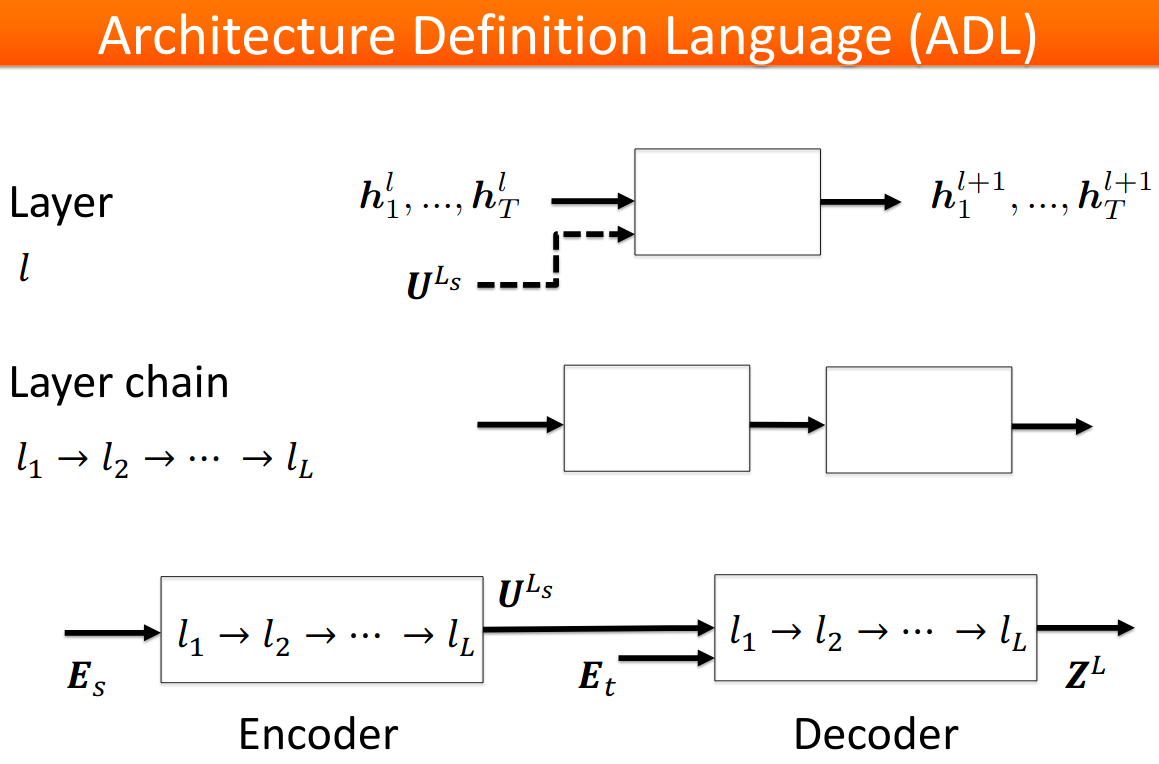
\includegraphics[width=\textwidth]{ADL.png}\\
            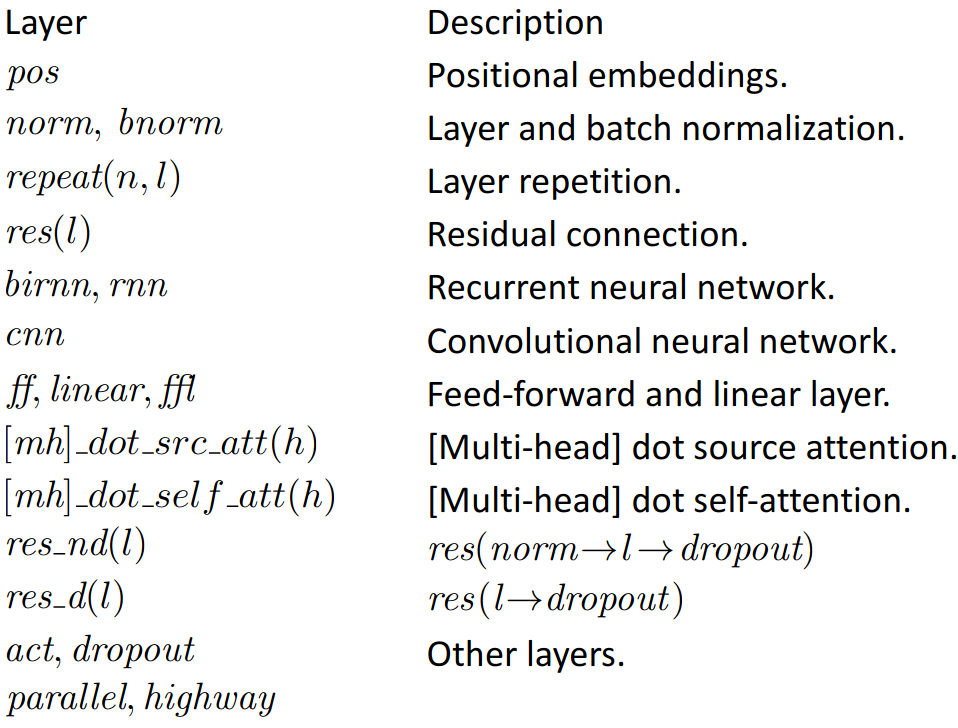
\includegraphics[width=\textwidth]{ADL_def.png}
        \end{column}
\end{columns}
\end{frame}

\begin{frame}
    \frametitle{Architecture Definition Language (ADL)}
    \begin{columns}
        \begin{column}{0.49\paperwidth}
            \underline{Fixed Positional Embeddings}
            \[
                pos(\textbf{h}_t) = dropout(\sqrt{d}\textbf{h}_t+\textbf{p}_t)
            \]
            \underline{Gated Linear Unit (GLU)}
            \[
                glu([\textbf{h}_A;\textbf{h}_B]) =
                \textbf{h}_A\otimes\sigma(\textbf{h}_B)
            \]
            \underline{Dot Product Attention}
            \[
                dot\_att(\textbf{Q},\textbf{K},\textbf{V},s)=
                softmax(\frac{\textbf{QK}^T}{\sqrt{s}})\textbf{V}
            \]
        \end{column}
        \begin{column}{0.49\paperwidth}
            \underline{Layer Normalization}
            \[
                nrom(\textbf{h}_t) = \frac{\textbf{g}}{\sigma_t}\otimes
                (\textbf{h}_t - \mu_t) + \textbf{b}
            \]
            \[
                \mu_t = \frac1d\textbf{h}_{t,j}   
                \hspace{1em}
                \sigma_t = \sqrt{\frac1d(\textbf{h}_{t,j} - \mu_j)^2}
            \]
            \underline{Residual Layer}
            \[
                res(\textbf{h}_t,l) = \textbf{h}_t + l(\textbf{h}_t
            \]
        \end{column}
    \end{columns}
\end{frame}

\begin{frame}
    \frametitle{Architecture Definition Language (ADL)}
    \vspace{-1em}
    \underline{Transformer}\\
    Encoder
    \vspace{-1.5em}
    \[
        t_{enc} = res\_nd(mh\_dot\_self\_attn)\rightarrow res\_nd(ffl)
    \]
    Decoder
    \\$t_{dec} = $
    \vspace{-1em}
    \[
        res\_nd(mh\_dot\_self\_attn)\rightarrow
        res\_nd(mh\_dot\_src\_att)\rightarrow res\_nd(ffl)
    \]
    \underline{RNN}
    \vspace{-1em}
    \begin{align*}
        rnn(\textbf{h}_t) &= f_{rnn\_o}(\textbf{h}_t,\textbf{s}_{t-1})\\
        \textbf{s}_t &= f_{rnn\_h}(\textbf{h}_t,\textbf{s}_{t-1})
    \end{align*}
    \underline{Convolution}
    \vspace{-1em}
    \[
        cnn(\textbf{H},v,k) =
        v(\textbf{W}[\textbf{h}_{i-\lfloor{k/2}\rfloor};
        \dots\;
        \textbf{h}_{i+\lfloor{k/2}\rfloor} ]+\textbf{b})
    \]
\end{frame}
